\documentclass{standalone}
\usepackage{tikz}
\usetikzlibrary{patterns, positioning}


\begin{document}
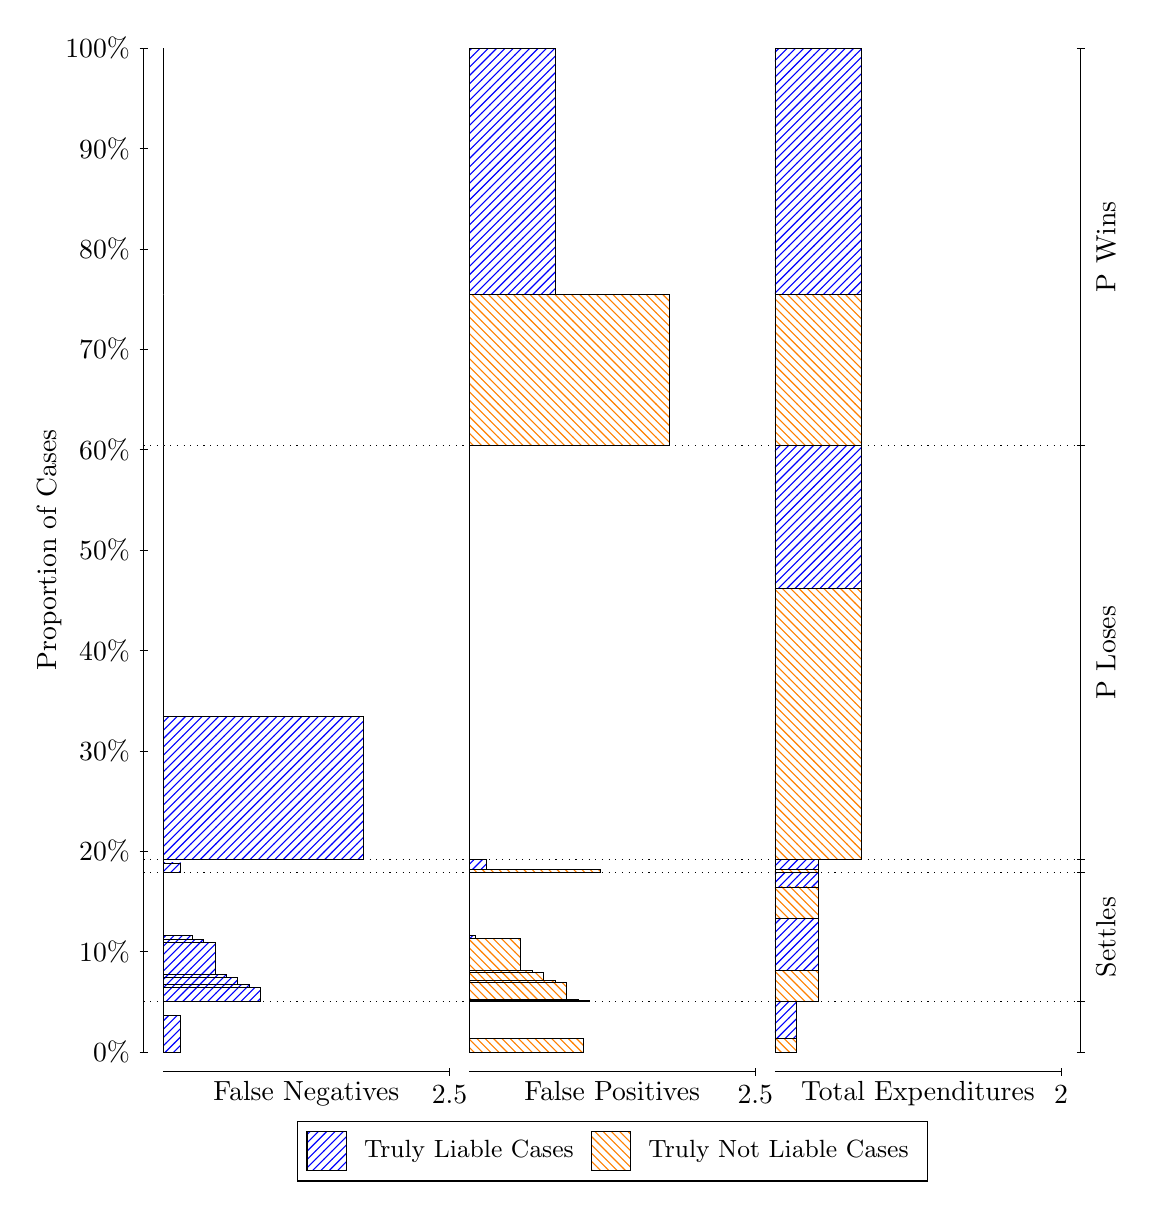
\begin{tikzpicture}
\draw[black, very thin] (1.5,1.75) -- (1.5,14.5);
\node[rotate=90, text=black, anchor=center] at (0.3, 8.125) {Proportion of Cases};
\draw[black, very thin] (1.45,1.75) -- (1.55,1.75);
\node[text=black, anchor=east] at (1.45, 1.75) {0\%};
\draw[black, very thin] (1.45,3.025) -- (1.55,3.025);
\node[text=black, anchor=east] at (1.45, 3.025) {10\%};
\draw[black, very thin] (1.45,4.3) -- (1.55,4.3);
\node[text=black, anchor=east] at (1.45, 4.3) {20\%};
\draw[black, very thin] (1.45,5.575) -- (1.55,5.575);
\node[text=black, anchor=east] at (1.45, 5.575) {30\%};
\draw[black, very thin] (1.45,6.85) -- (1.55,6.85);
\node[text=black, anchor=east] at (1.45, 6.85) {40\%};
\draw[black, very thin] (1.45,8.125) -- (1.55,8.125);
\node[text=black, anchor=east] at (1.45, 8.125) {50\%};
\draw[black, very thin] (1.45,9.4) -- (1.55,9.4);
\node[text=black, anchor=east] at (1.45, 9.4) {60\%};
\draw[black, very thin] (1.45,10.675) -- (1.55,10.675);
\node[text=black, anchor=east] at (1.45, 10.675) {70\%};
\draw[black, very thin] (1.45,11.95) -- (1.55,11.95);
\node[text=black, anchor=east] at (1.45, 11.95) {80\%};
\draw[black, very thin] (1.45,13.225) -- (1.55,13.225);
\node[text=black, anchor=east] at (1.45, 13.225) {90\%};
\draw[black, very thin] (1.45,14.5) -- (1.55,14.5);
\node[text=black, anchor=east] at (1.45, 14.5) {100\%};

\draw[black, very thin] (13.4,1.75) -- (13.4,14.5);
\draw[black, very thin] (13.35,1.75) -- (13.45,1.75);
\node[anchor=west] at (13.35, 1.75) {};
\draw[black, very thin] (13.35,2.3884) -- (13.45,2.3884);
\node[anchor=west] at (13.35, 2.3884) {};
\draw[black, very thin] (13.35,4.0295) -- (13.45,4.0295);
\node[anchor=west] at (13.35, 4.0295) {};
\draw[black, very thin] (13.35,4.1944) -- (13.45,4.1944);
\node[anchor=west] at (13.35, 4.1944) {};
\draw[black, very thin] (13.35,9.452) -- (13.45,9.452);
\node[anchor=west] at (13.35, 9.452) {};
\draw[black, very thin] (13.35,14.5) -- (13.45,14.5);
\node[anchor=west] at (13.35, 14.5) {};

\draw[black, very thin, pattern color=blue, pattern=north east lines] (1.75,1.75) rectangle (1.968,2.2131);
\draw[black, very thin, pattern color=orange, pattern=north west lines] (1.75,2.2131) rectangle (1.75,2.3884);
\draw[black, very thin, pattern color=blue, pattern=north east lines] (1.75,2.3884) rectangle (2.9853,2.5717);
\draw[black, very thin, pattern color=blue, pattern=north east lines] (1.75,2.5717) rectangle (2.84,2.6036);
\draw[black, very thin, pattern color=blue, pattern=north east lines] (1.75,2.6036) rectangle (2.6947,2.6966);
\draw[black, very thin, pattern color=blue, pattern=north east lines] (1.75,2.6966) rectangle (2.5493,2.7305);
\draw[black, very thin, pattern color=blue, pattern=north east lines] (1.75,2.7305) rectangle (2.404,3.1417);
\draw[black, very thin, pattern color=blue, pattern=north east lines] (1.75,3.1417) rectangle (2.2587,3.1823);
\draw[black, very thin, pattern color=blue, pattern=north east lines] (1.75,3.1823) rectangle (2.1133,3.2299);
\draw[black, very thin, pattern color=orange, pattern=north west lines] (1.75,3.2299) rectangle (1.75,4.0295);
\draw[black, very thin, pattern color=blue, pattern=north east lines] (1.75,4.0295) rectangle (1.968,4.1521);
\draw[black, very thin, pattern color=orange, pattern=north west lines] (1.75,4.1521) rectangle (1.75,4.1944);
\draw[black, very thin, pattern color=blue, pattern=north east lines] (1.75,4.1944) rectangle (4.2933,6.0138);
\draw[black, very thin, pattern color=orange, pattern=north west lines] (1.75,6.0138) rectangle (1.75,9.452);
\draw[black, very thin, pattern color=orange, pattern=north west lines] (1.75,9.452) rectangle (1.75,11.372);
\draw[black, very thin, pattern color=blue, pattern=north east lines] (1.75,11.372) rectangle (1.75,14.5);
\draw[black, very thin, pattern color=orange, pattern=north west lines] (5.6333,1.75) rectangle (7.0867,1.9252);
\draw[black, very thin, pattern color=blue, pattern=north east lines] (5.6333,1.9252) rectangle (5.6333,2.3884);
\draw[black, very thin, pattern color=orange, pattern=north west lines] (5.6333,2.3884) rectangle (7.1593,2.4024);
\draw[black, very thin, pattern color=orange, pattern=north west lines] (5.6333,2.4024) rectangle (7.014,2.4179);
\draw[black, very thin, pattern color=orange, pattern=north west lines] (5.6333,2.4179) rectangle (6.8687,2.6291);
\draw[black, very thin, pattern color=orange, pattern=north west lines] (5.6333,2.6291) rectangle (6.7233,2.6616);
\draw[black, very thin, pattern color=orange, pattern=north west lines] (5.6333,2.6616) rectangle (6.578,2.7559);
\draw[black, very thin, pattern color=orange, pattern=north west lines] (5.6333,2.7559) rectangle (6.4327,2.7872);
\draw[black, very thin, pattern color=orange, pattern=north west lines] (5.6333,2.7872) rectangle (6.2873,3.1879);
\draw[black, very thin, pattern color=blue, pattern=north east lines] (5.6333,3.1879) rectangle (5.706,3.2355);
\draw[black, very thin, pattern color=blue, pattern=north east lines] (5.6333,3.2355) rectangle (5.6333,4.0295);
\draw[black, very thin, pattern color=orange, pattern=north west lines] (5.6333,4.0295) rectangle (7.3047,4.0718);
\draw[black, very thin, pattern color=blue, pattern=north east lines] (5.6333,4.0718) rectangle (5.8513,4.1944);
\draw[black, very thin, pattern color=orange, pattern=north west lines] (5.6333,4.1944) rectangle (5.6333,7.6326);
\draw[black, very thin, pattern color=blue, pattern=north east lines] (5.6333,7.6326) rectangle (5.6333,9.452);
\draw[black, very thin, pattern color=orange, pattern=north west lines] (5.6333,9.452) rectangle (8.1767,11.372);
\draw[black, very thin, pattern color=blue, pattern=north east lines] (5.6333,11.372) rectangle (6.7233,14.5);
\draw[black, very thin, pattern color=orange, pattern=north west lines] (9.5167,1.75) rectangle (9.7892,1.9252);
\draw[black, very thin, pattern color=blue, pattern=north east lines] (9.5167,1.9252) rectangle (9.7892,2.3884);
\draw[black, very thin, pattern color=orange, pattern=north west lines] (9.5167,2.3884) rectangle (10.062,2.7872);
\draw[black, very thin, pattern color=blue, pattern=north east lines] (9.5167,2.7872) rectangle (10.062,3.4453);
\draw[black, very thin, pattern color=orange, pattern=north west lines] (9.5167,3.4453) rectangle (10.062,3.8461);
\draw[black, very thin, pattern color=blue, pattern=north east lines] (9.5167,3.8461) rectangle (10.062,4.0295);
\draw[black, very thin, pattern color=orange, pattern=north west lines] (9.5167,4.0295) rectangle (10.062,4.0718);
\draw[black, very thin, pattern color=blue, pattern=north east lines] (9.5167,4.0718) rectangle (10.062,4.1944);
\draw[black, very thin, pattern color=orange, pattern=north west lines] (9.5167,4.1944) rectangle (10.607,7.6326);
\draw[black, very thin, pattern color=blue, pattern=north east lines] (9.5167,7.6326) rectangle (10.607,9.452);
\draw[black, very thin, pattern color=orange, pattern=north west lines] (9.5167,9.452) rectangle (10.607,11.372);
\draw[black, very thin, pattern color=blue, pattern=north east lines] (9.5167,11.372) rectangle (10.607,14.5);
\draw[black, dotted] (1.5,2.3884) -- (13.4,2.3884);
\draw[black, dotted] (1.5,4.0295) -- (13.4,4.0295);
\draw[black, dotted] (1.5,4.1944) -- (13.4,4.1944);
\draw[black, dotted] (1.5,9.452) -- (13.4,9.452);
\draw[black, very thin] (1.75,1.5) -- (5.3833,1.5);
\node[text=black, anchor=north] at (3.5667, 1.5) {False Negatives};
\draw[black, very thin] (5.3833,1.45) -- (5.3833,1.55);
\node[text=black, anchor=north] at (5.3833, 1.45) {2.5};

\draw[black, very thin] (5.6333,1.5) -- (9.2667,1.5);
\node[text=black, anchor=north] at (7.45, 1.5) {False Positives};
\draw[black, very thin] (9.2667,1.45) -- (9.2667,1.55);
\node[text=black, anchor=north] at (9.2667, 1.45) {2.5};

\draw[black, very thin] (9.5167,1.5) -- (13.15,1.5);
\node[text=black, anchor=north] at (11.333, 1.5) {Total Expenditures};
\draw[black, very thin] (13.15,1.45) -- (13.15,1.55);
\node[text=black, anchor=north] at (13.15, 1.45) {2};


\node[text=black, centered, rotate=90] at (13.72, 3.2089) {Settles};

\node[text=black, centered, rotate=90] at (13.72, 6.8232) {P Loses};
\node[text=black, centered, rotate=90] at (13.72, 11.976) {P Wins};

\draw (7.449999999999999,1.5) node[draw=none] (baseCoordinate) {};
\begin{scope}[align=center]
        \matrix[scale=0.5, draw=black, below=0.5cm of baseCoordinate, nodes={draw}, column sep=0.1cm]{
            \node[rectangle, draw, minimum width=0.5cm, minimum height=0.5cm, pattern color=blue, pattern=north east lines] {}; &
            \node[draw=none, font=\small, text=black] (B) {Truly Liable Cases}; &
            \node[rectangle, draw, minimum width=0.5cm, minimum height=0.5cm, pattern color=orange, pattern=north west lines] {}; &
            \node[draw=none, font=\small, text=black] (B) {Truly Not Liable Cases}; \\
            };
\end{scope}

\end{tikzpicture}
\end{document}